\documentclass[varwidth=\maxdimen]{standalone}
\usepackage{booktabs}
\usepackage{multirow}
\usepackage{mathtools}
\usepackage{array}
\usepackage[table]{xcolor}
\usepackage{tikz}
\usepackage{moresize}

\DeclarePairedDelimiter\ceil{\lceil}{\rceil}
\DeclarePairedDelimiter\floor{\lfloor}{\rfloor}
\def\checkmark{\tikz\fill[scale=0.4](0,.35) -- (.25,0) -- (1,.7) -- (.25,.15) -- cycle;} 

\begin{document}
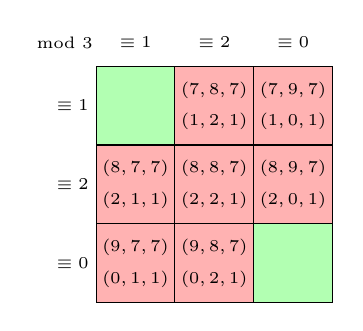
\begin{tikzpicture}

\draw[gray,fill=red!30] (1,1) rectangle (2,2);
\draw[gray,fill=red!30] (2,1) rectangle (3,2);
\draw[gray,fill=red!30] (1,2) rectangle (2,3);
\draw[gray,fill=red!30] (3,2) rectangle (4,3);
\draw[gray,fill=red!30] (2,3) rectangle (3,4);
\draw[gray,fill=green!30] (3,1) rectangle (4,2);
\draw[gray,fill=red!30] (3,3) rectangle (4,4);

\draw[gray,fill=red!30] (2,2) rectangle (3,3);
\draw[gray,fill=green!30] (1,3) rectangle (2,4);

\draw[] (1,1) grid (4,4);

\node[font=\ssmall] at (0.6,4.3) {mod 3};

\node[font=\ssmall] at (1.5,4.3) {$\equiv 1$};
\node[font=\ssmall] at (2.5,4.3) {$\equiv 2$};
\node[font=\ssmall] at (3.5,4.3) {$\equiv 0$};

\node[font=\ssmall] at (0.7,3.5) {$\equiv 1$};
\node[font=\ssmall] at (0.7,2.5) {$\equiv 2$};
\node[font=\ssmall] at (0.7,1.5) {$\equiv 0$};

\node[font=\ssmall] at (2.5,3.7) {$(7,8,7)$};
\node[font=\ssmall] at (2.5,3.3) {$(1,2,1)$};

\node[font=\ssmall] at (3.5,3.7) {$(7,9,7)$};
\node[font=\ssmall] at (3.5,3.3) {$(1,0,1)$};

\node[font=\ssmall] at (3.5,2.7) {$(8,9,7)$};
\node[font=\ssmall] at (3.5,2.3) {$(2,0,1)$};

\node[font=\ssmall] at (2.5,2.7) {$(8,8,7)$};
\node[font=\ssmall] at (2.5,2.3) {$(2,2,1)$};

\node[font=\ssmall] at (2.5,1.7) {$(9,8,7)$};
\node[font=\ssmall] at (2.5,1.3) {$(0,2,1)$};

\node[font=\ssmall] at (1.5,1.7) {$(9,7,7)$};
\node[font=\ssmall] at (1.5,1.3) {$(0,1,1)$};

\node[font=\ssmall] at (1.5,2.7) {$(8,7,7)$};
\node[font=\ssmall] at (1.5,2.3) {$(2,1,1)$};
\end{tikzpicture}
\end{document}